%!TEX TS-program = pdflatex
% wikinger workbook
\documentclass[12pt,a4paper,ngerman,openany]{book}
\usepackage{graphicx}
\usepackage[hang,splitrule]{footmisc}
\usepackage[ngerman]{babel}
\usepackage[parfill]{parskip}
\usepackage[T1]{fontenc}
\usepackage[utf8]{inputenc}
\usepackage{afterpage}
\usepackage{amssymb}
\usepackage{booktabs}
\usepackage{chngcntr}
\usepackage{color}
\usepackage{etoolbox}
\usepackage{fancyhdr}
\usepackage{geometry}
\usepackage{graphicx}
\usepackage{hyphenat}
\usepackage{lettrine}
\usepackage{paralist}
\usepackage{pdfpages}
\usepackage{setspace}
\usepackage{tabularx}
\usepackage{tcolorbox}
\usepackage{titlesec}
\usepackage{wrapfig}
\usepackage[final,stretch=10,protrusion=true,tracking=true,expansion=true]{microtype}
\PassOptionsToPackage{hyphens}{url}\usepackage{hyperref}

\renewcommand{\familydefault}{pplj} 
\renewcommand{\footnoterule}{\vspace{0.5em}\noindent{\line(1,0){120}} \vspace{.5em} }
\renewcommand{\LettrineFontHook}{\initfamily}
\newcommand{\flettrine}[2]{\lettrine[lines=2, depth=0, loversize=0.25, nindent=0.69pt, lraise=0.15]{\initfamily{#1}}{#2}}
\newcommand{\estcab}[1]{\itshape{\nouppercase #1}}
\newcommand*\initfamily{\usefont{U}{GotIn}{xl}{n}}
\newcommand\blankpage{\null \thispagestyle{empty} \addtocounter{page}{-1} \newpage}
\newcommand{\aufgaben}[1]{
  \begin{tcolorbox}
    \textbf{Aufgaben}
    \begin{enumerate}
      #1
    \end{enumerate}
  \end{tcolorbox}
} % exercises module
\newcommand{\erklaer}[2]{\leavevmode\marginpar{\footnotesize \textbf{#1:}\\#2}\ignorespaces \textit{#1}} % explanations in the margin
\newcommand{\timage}[1]{\framebox{\includegraphics[height=10em]{#1}}} % image in table
\newcommand{\ttext}[1]{\hline\vspace*{-10em}#1} % text in table

\geometry{
tmargin=0cm,bmargin=3cm,
lmargin=3cm,rmargin=2cm,
headheight=1.5cm,headsep=0.8cm,
footskip=1cm}

\setlength{\parskip}{1.3ex plus 0.2ex minus 0.2ex}
\setlength{\parindent}{0cm}
\setlength{\footnotemargin}{0.3cm}
\setlength{\footnotesep}{0.4cm} 
\addtolength{\footskip}{0.5cm}
\setdefaultleftmargin{0.667cm}{}{}{}{}{}
\setlength{\fboxsep}{5pt}
\setlength{\fboxrule}{0pt}

\newcommand{\fchapter}[1]{\chapter{#1}\thispagestyle{chapterstyle}}

\fancyhf{}

\fancypagestyle{chapterstyle}{ % für kapitelbeginn
  \renewcommand{\headrulewidth}{0pt}
  \fancyhead{}
  \fancyfoot[LE,RO]{\thepage}
}

\fancypagestyle{normalpage}{ % normale seiten
  \fancyhead[LE,RO]{\textit{\nouppercase{\leftmark}}}
  \fancyhead[RE,LO]{\textit{\nouppercase{\rightmark}}}
  \fancyfoot[LE,RO]{\thepage}
}

\pagestyle{normalpage}
\renewcommand{\chaptermark}[1]{\markboth{#1}{}}
\renewcommand{\sectionmark}[1]{\markright{#1}{}}

\input GotIn.fd % lettrine font
\setstretch{1.125} % 1.125x line spacing
\hyphenation{Mathe-matik wieder-gewinnen} % silbentrennung
\graphicspath{{./img/}}

% space between 'chap #' and chap-title (https://latex.org/forum/viewtopic.php?t=21666)
\titleformat{\chapter}[display]{\normalfont\huge\bfseries}{\chaptertitlename\ \thechapter}{0pt}{\Huge}

% für lückentext
\newlength{\diebox}
\newcommand{\luecke}[1]{\settowidth{\diebox}{#1}\raisebox{-1.0ex}{\parbox{2.7\diebox}{\dotfill}}}

%%%%%%%%%%%%%%%%%%%%%%%%%%%%%%%%%%%%%%%%%%%%%
%%%%%%%%%%%%%%%%%%%%%%%%%%%%%%%%%%%%%%%%%%%%%

% doppelseitig: mit long edge drucken
% pdfbook2 -t 0 -b 0 -i 0 -o 0 main.pdf

\begin{document}

\includepdf[pages=-]{wikinger-workbook-front.pdf}
\thispagestyle{empty}
\newpage

\afterpage{\blankpage}
\tableofcontents
\thispagestyle{empty}

\newgeometry{top=2cm, bottom=2.5cm,% for text
outer=3.75cm, inner=2cm,%
heightrounded, marginparwidth=2.8cm,%
marginparsep=0.3cm}

\fchapter{Einleitung}

\section{Wer waren die Wikinger?}

\flettrine{D}{er Wikinger:} Einen eisernen Helm auf dem Kopf, ein schweres Schwert in den Händen, plumpe Kleider am Körper und direkt auf dem Weg zum nächsten Raubzug.
Klingt schräg, aber ist doch das Bild, das jedem bei dem Gedanken an die alten Wikinger in den Kopf kommt. Die Frage ist jedoch: Stimmt dieses vermeintliche Wissen über die Wikinger?
Waren sie wirklich so barbarisch? Waren die Wikinger kopflose Kämpfer, denen es nur nach Reichtum schmachtete?\\\\
Die Antwort ist gar nicht so einfach. Man könnte sagen ja und nein. Beginnen wir ganz am Anfang. Das Wikingerzeitalter begann im Jahr 793 n. Chr. und erstreckte sich bis zum Jahr 1066 n. Chr.
Verschiedenste Menschen kamen verstreut aus dem skandinavischen Raum, also Norwegen, Schweden und Dänemark, es war also ein Zusammentreffen unterschiedlichster Kulturen und Individuen.
Und diese waren keinesfalls ausnahmslos Krieger oder Kämpfer, in dem bunten Gemisch aus Menschen fanden sich sowohl zahlreiche Händler, als auch Bauern, genauso wie Seemänner und unter anderem auch nur einfache Siedler.
Sie begannen die weiten Gewässer zu erkunden, neues Gebiet zu entdecken und auch um ihr Überleben zu kämpfen. Es entwickelten sich gesellschaftliche Stämme und Dörfer.

\begin{wrapfigure}{l}{0.35\textwidth}
  \centering
  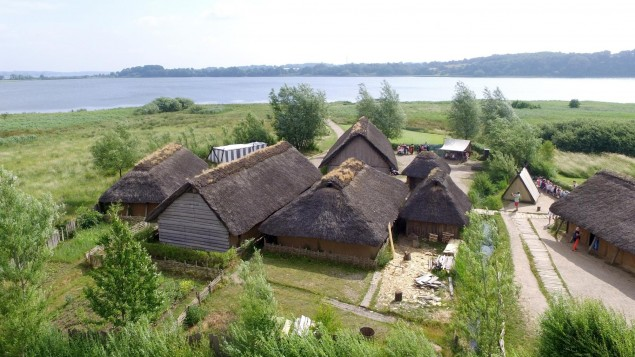
\includegraphics[width=0.33\textwidth]{haithabu.jpg}
  Das Wikingerdorf Haithabu.
\end{wrapfigure}
%TODO hier den newline fixen
Ein Beispiel dafür kann man noch heute fast eintausend Jahre später in der Nähe von Schleswig begutachten: Das 770 n. Chr. gegründete Haithabu. Zu damaliger Zeit war dieser zentrale,
zwischen der Nord- und Ostsee gelegene Ort ein wichtiger Handelsort und Hauptumschlagplatz für die Wikinger aus Skandinavien, dem Baltikum und Westeuropa. Mit verschiedenen Rohstoffen wie beispielsweise Eisen,
das zu jener Zeit sogar recht selten und kostbar war, wurden Waffen hergestellt, mit denen Kämpfe ausgetragen wurden.\\ 
Auf ihren Reisen auf dem Meer entdeckten sie nicht nur neues Gebiet, sondern trafen auch auf andere Gesellschaften. Bei diesen Begegnungen gingen sie rücksichtslos vor, raubten andere Völker aus und zerstörten anderes Eigentum.
Solche Kämpfe waren üblich. Außerdem versklavten die Wikinger die Überlebenden und nahmen sie mit auf ihre Raubzüge. Andere Sklaven wurden von diesen in das Heimatdorf der Wikinger gebracht, damit jene dort bei den zu erledigenden Aufgaben halfen.
Zum anderen waren die Wikinger auch Händler, die mit verschiedensten Waren auf Reisen aber auch im Heimatdorf handelten.\\
Auf der anderen Seite sollte durchaus erwähnt werden, dass die Gesellschaft der Wikinger für die damalige Zeit recht fortgeschritten war. Zum Beispiel gab es die Möglichkeit, seine Meinung in der Öffentlichkeit relativ frei zu äußern.
Eigentlich kann man aber nicht von einer Gesellschaft sprechen, sondern eher von mehreren sogenannten Sippen und Familienverbänden. In einer Sippe lebten teilweise bis zu drei Generationen gemeinsam: Die Großeltern, die Eltern und die Kinder.
Zusammen hausten sie in einem großen Raum, welchen wir heute als das typische Haus der Wikinger bezeichnen. Gerade Kinder und Eltern waren einander im Alltag wichtige Partner. Während Mutter und Vater ihre Aufgaben erledigten,
lernten Tochter und Sohn von ihnen und halfen ihren Eltern. Somit stand die Zukunft für das jeweilige Geschlecht bereits früh fest; das Mädchen lernte die Arbeiten der Mutter kennen, zum Beispiel die Fertigung von Kleidung, und mit der Zeit auch, sie zu übernehmen.
Genauso wie die Jungen auf der anderen Seite sich die Tätigkeiten der Väter aneigneten, zum Beispiel der Umgang mit der Waffe auf Raubzügen, auf die sie ihre Väter manchmal begleiteten.\\
Auf politischer Ebene musste man den Wikingern sicherlich auch eine gewisse Anerkennung entgegenbringen, denn Gesetze und auch Rechte waren sehr wichtige Werte für die Wikinger. Zum Beispiel tagten die Wikinger regelmäßig zusammen in Form einer Volksversammlung,
welche das \glqq Thing\grqq{} genannt wurde. Die Termine waren festgelegt und die Versammlungen, in denen man über politische Angelegenheiten, Recht und Gesetz abstimmte und beriet, fanden immer unter freiem Himmel statt.\\
Außerdem war eine Hochzeit zwischen Mann und Frau offiziell durchaus möglich, genauso aber auch, sich wieder voneinander scheiden zu lassen. 
Für die Zivilisiertheit der Wikinger sprach außerdem ihre Intention, sich nach außen hin gut und ordentlich zu präsentieren, denn die Wikinger legten Wert auf ihr Äußeres. Dazu zählte die Art sich zu kleiden,
ein gewisses Maß an Hygiene und auch Schmuck war bereits damals ein wichtiges Accessoire. Zahlreiche Goldschmiedearbeiten und Runensteine, die man später in vielen der Gräbern fand, zeugten von der geistigen Feinheit der Wikinger. 

\aufgaben {
  \item Lies den Text und notiere dir Stichworte, um dir einen Überblick zu schaffen.
}

\pagebreak

\section{Zeitlicher Überblick}

\begin{tcolorbox}[sharp corners, title=08. Juni 793]
Erster historisch festgehaltene Angriff auf die Abtei Lindisfarne in Northumberland, Nordengland. Hier wurden Reliquien des Heiligen Cuthbert aufbewahrt. Die angreifenden Wikinger plünderten das Kloster und legten es in Schutt und Asche.\\
Bereits vorher gab es schon Aktivitäten, jedoch wurden diese nicht historisch festgehalten.
\end{tcolorbox}

\begin{tcolorbox}[sharp corners, title=Ungefähr 800 bis 850]
In dieser Anfangszeit gab es meist unkoordinierte Angriffe auf Orte ohne gute Verteidigung und mit viel Reichtum, wo es also viel potenzielle Beute gab. Oft wurden Klöster, Abteien und offene Städte (Städte ohne Verteidigung) überfallen.
\end{tcolorbox}

\begin{tcolorbox}[sharp corners, title=Ungefähr 850 bis 900]
In dieser sehr aktiven Phase wurden die Wikinger sich langsam ihres kriegerischen Potenzials bewusst. Die Angriffe wurden jetzt besser geplant, liefen koordinierter ab und die allgemeine Bevölkerung anderer Länder hatte große Angst vor den Plünderern.
Jedoch wurden stärkere Nationen, die sich gegen den Wikingeransturm verteidigt haben, wie zum Beispiel Südengland, zunehmend in Ruhe gelassen. Daraus kann man erkennen, dass die Wikinger keine richtigen Kriegsherren waren und auch öfters größere Schlachten verloren haben. Zumal das Wikingervolk auch zu klein war, um Truppen aufzustellen, die groß genug wären, um sich mit den stärkeren Gegnern zu messen.
In dieser Zeit forderten die Wikinger auch das sogenannte \textit{danegeld} (\glqq Bezahlung an die Dänen\grqq{}). Dieses immer steigende Schutzgeld (eine durch Androhung von Gewalt erpresste regelmäßige Zahlung) wurde gezahlt, damit die Wikinger Dänemark nicht überfallen.
In dieser Zeit kristallisierten sich auch die wichtigsten Handelsrouten heraus, wie zum Beispiel die West- und Nordroute.
\end{tcolorbox}

\begin{tcolorbox}[sharp corners, title=Ungefähr 900 bis 980]
Zunehmend entstanden feste Niederlassungen und Territorien, vor allem in Skandinavien, aber auch beispielsweise in der Normandie (Nordwestfrankreich), Grönland, in Teilen Englands und Novgorod (Westrussland), zu welchen auch Handelsrouten bestanden. Falls die Wikinger sich aber, wie oben teilweise genannt, in anderen Ländern niederließen, mussten sie auch die dortigen Gesetze befolgen und sich dort eingliedern, wozu auch der Verteidigungsdienst für das \glqq neue\grqq{} Vaterland zählte. Dadurch verschwindet in diesen Fällen \glqq der Wikinger\grqq{} nach ein paar Generationen aus dem Gesellschaftsbild.
\end{tcolorbox}

\begin{tcolorbox}[sharp corners, title=Ungefähr 980 bis 1066]
Hier ging es meist nur noch um die restlichen Wikinger im Nordwesten Dänemarks und Südosten Schwedens. In Dänemark versuchten sie, für eine kurze Zeit erfolgreich, die Herrschaft an sich zu reißen, während in Schweden lange Expeditionen nach Zentralasien gemacht wurden. Jedoch verloren die Wikinger zunehmend an Bedeutung, nicht nur weil das Wikingervolk immer kleiner wurde. Als größter Faktor für das \glqq Verschwinden\grqq{} des Wikingers ist die Christianisierung Nordeuropas zu nennen, durch welche auch zentrale Herrscher (Könige) großer Gebiete begünstigt wurden, zumal die einzelnen Wikingergruppen nie solche großen Gebiete kontrolliert haben, sondern eher lokale, kleinere Territorien beanspruchten.
\end{tcolorbox}

\vspace{0.66cm}

\aufgaben{
  \item Ordne die folgenden Szenarien den verschiedenen Zeitperioden zu.
}

\begin{itemize}
\item Björn und Helga bauen sich mit der Hilfe ihrer Familien ein Haus auf neuem Land.
\item Sven und einige Freunde aus dem Dorf lagern etwas Proviant für den morgigen Überfall auf ein kleines Kloster ein.
\item Sigmund und Thorleif arbeiten einen detaillierten Plan für einen Raubzug aus, an dem mehrere Dörfer beteiligt sind.
\item Der Bischof eines englisches Stifts bekommt zunehmend Angst, dass seine Abtei überfallen werden könnte.
\item Ein paar Wikinger bereiten sich auf eine lange Expedition nach Asien vor.
\item Der Jarl Olaf gibt seine Territorien auf und schließt sich dem neuen Königreich an.
\item Einige Königshäuser beginnen, den Wikingern Schutzgeld zu bezahlen.
\end{itemize}

\fchapter{Der typische Wikinger}

\section{Alltagskleidung}
\flettrine{D}{Das äussere Erscheinungsbild} war den Wikingern wichtig, weshalb ihre Kleidung gepflegt war und durch ihre hohe Wertigkeit in der Gesellschaft teilweise auch zum Ausdruck von Wohlstand genutzt wurde.\\
Als Alltagskleidung diente den Männern ein Hemd oder eine Tunika, welche zusammen mit einer lockeren Hose, die entweder unter den Knien geschnürt wurde oder locker bis zu den Knöcheln hing, getragen wurden. Um die Hüfte trugen sie einen Gürtel. Als Überwurf trugen sie einen Stoff, der einem Umhang ähnelte, befestigt mit einer Brosche. Die Schuhe bestanden aus einem robust geformten Leder, welches noch durch eine Sohle ergänzt wurde. Diese wurden um den Knöchel mit einer Kordel befestigt. Im Winter, wenn es kalt wurde, haben die Wikinger einen Pelzmantel angezogen. Als Kopfbedeckungen gab es Hüte oder Tücher, die auch von den Frauen getragen wurden.

\begin{wrapfigure}{r}{0.35\textwidth}
  \centering
  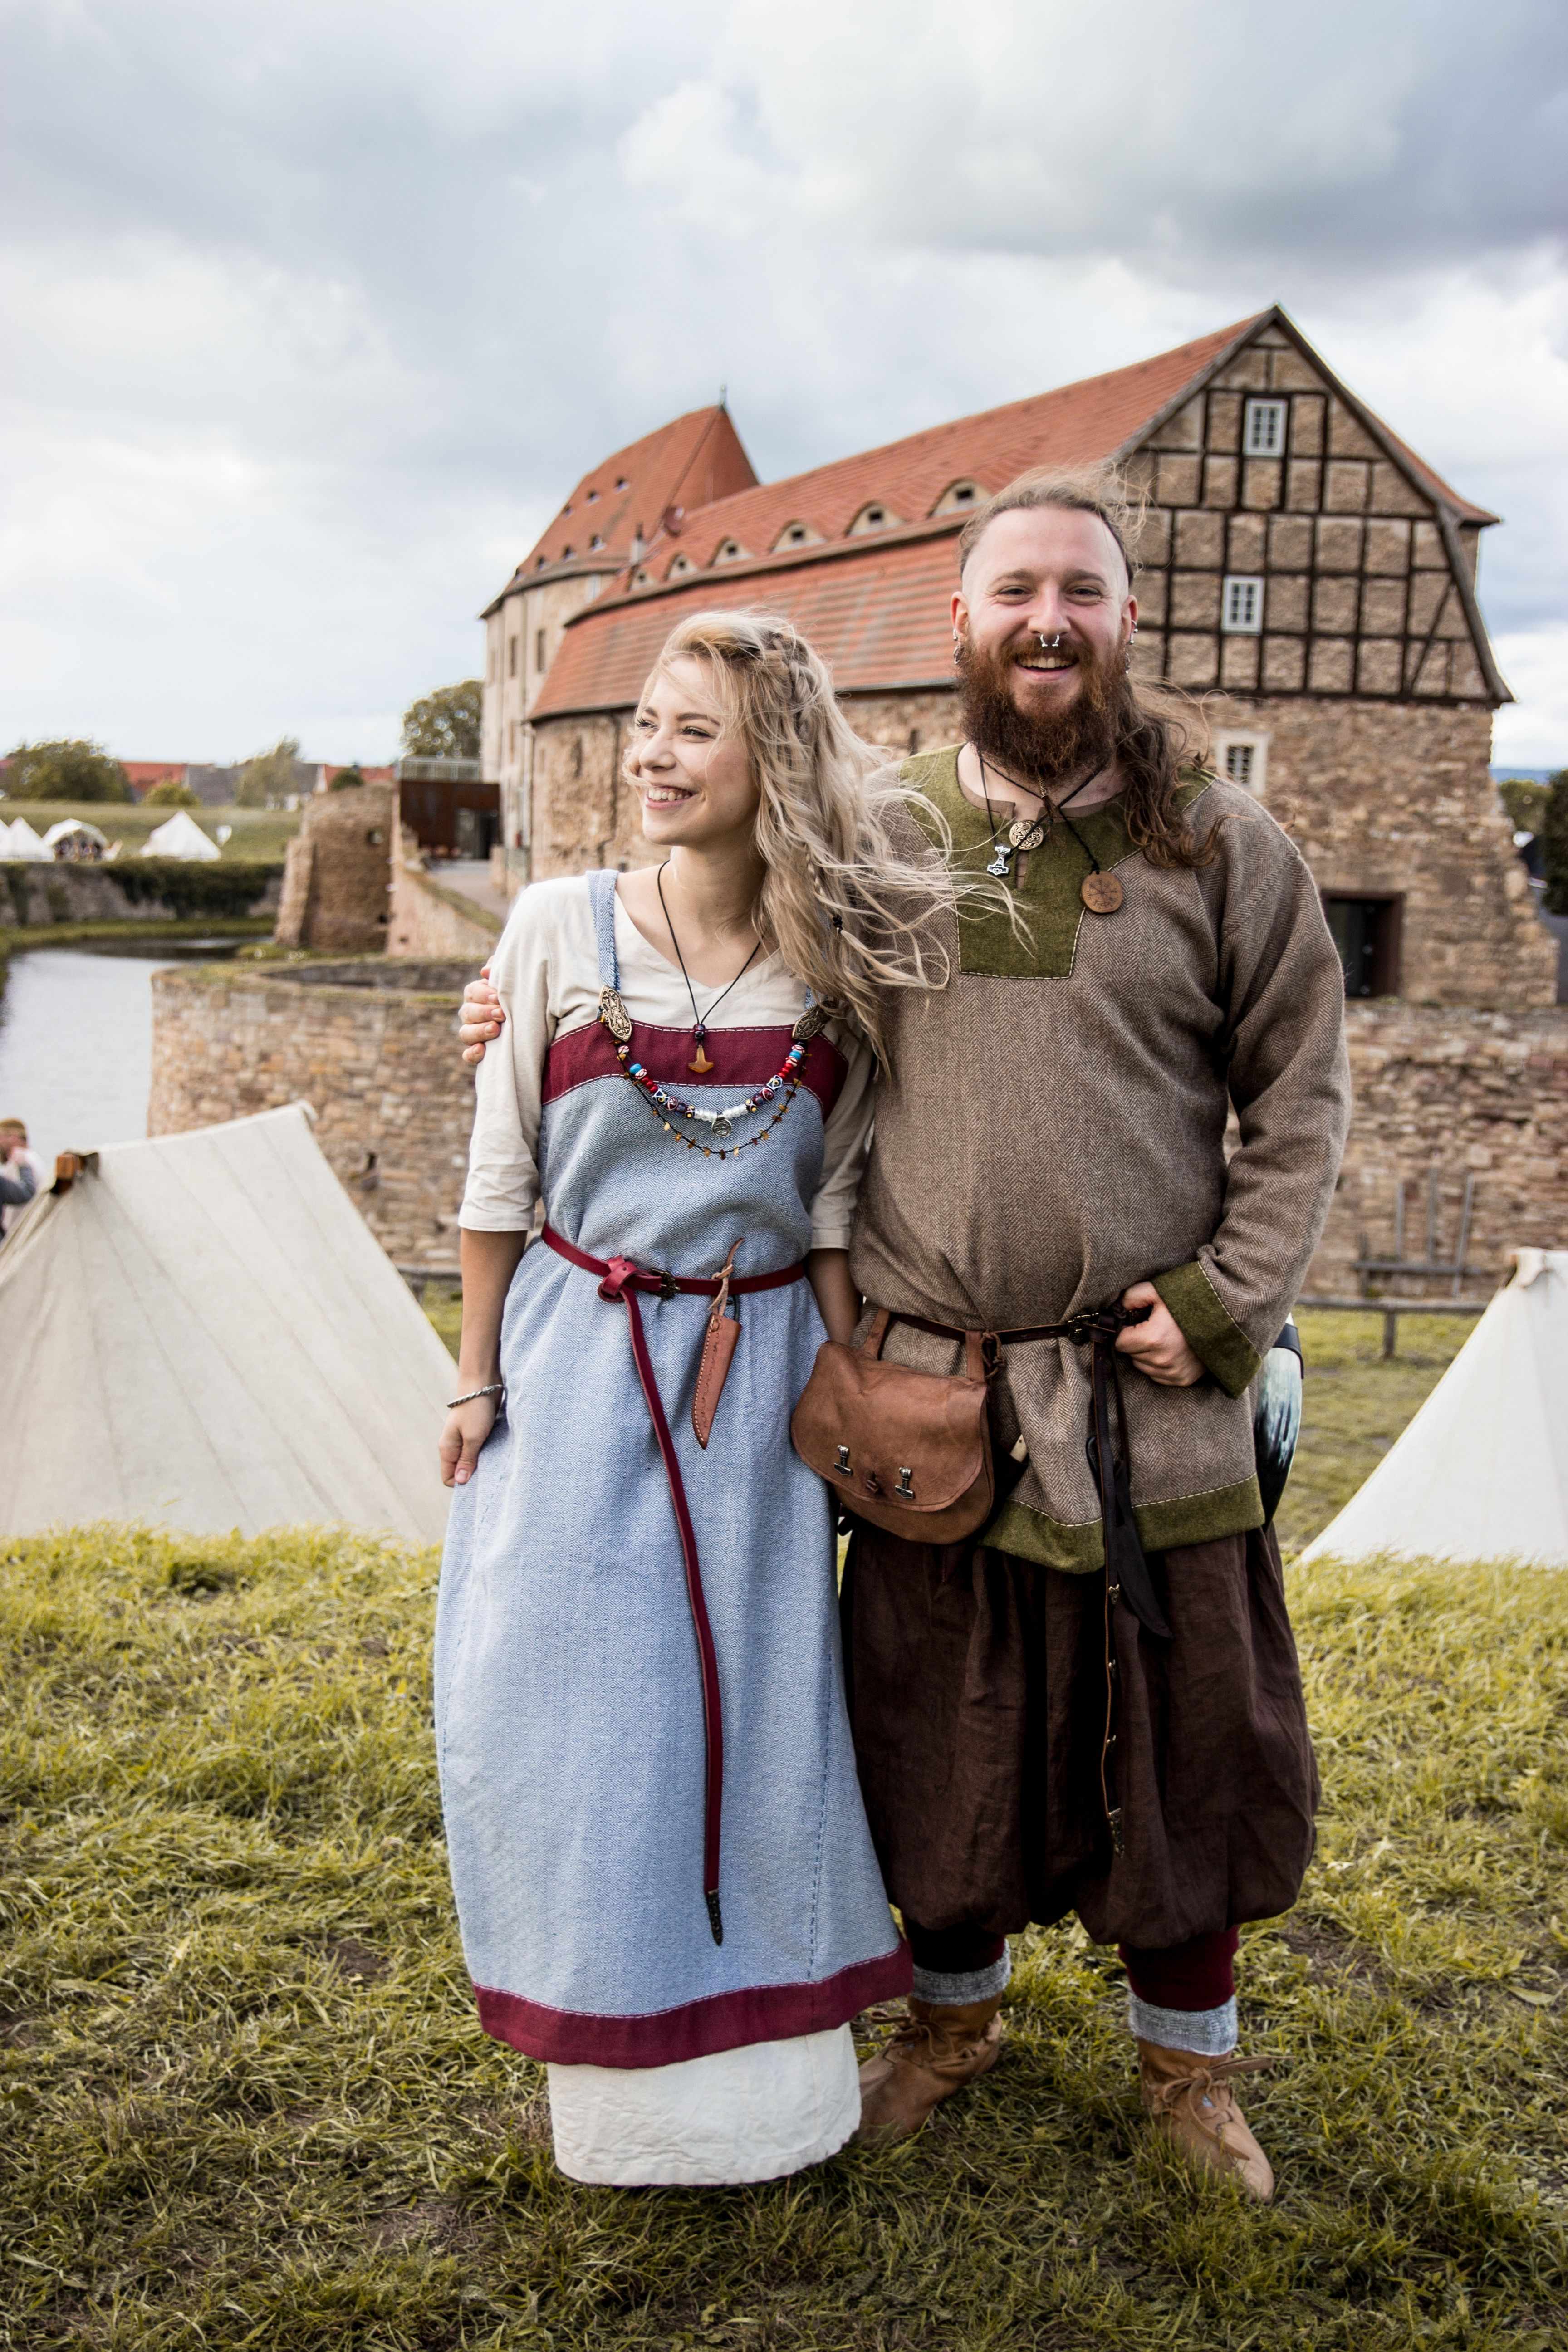
\includegraphics[width=0.29\textwidth]{kleidung.jpg}
  Typische Wikingerkleidung.
\end{wrapfigure}

Außerdem haben die Frauen im Alltag ein Gewand mit kurzen aber auch langen Ärmeln, das einem Kleid ähnelt, getragen, welches mit einer oder mehreren Schnallen über der Brust verschlossen wurde. Darüber haben die Frauen eine Schürze getragen. An dieser Schürze waren teilweise Broschen befestigt und auch an den Armen trugen sie einige Schmuckstücke. Bei den Frauen war die Farbe rot beliebt, während die Männer blau bevorzugten.\\
Die Kleidung wurde meist von den Frauen durch Weben oder Spinnen gefertigt, wobei sie häufig Wolle benutzten, die von den Tieren aus ihrem Dorf stammte. Aber auch Leinen oder Stoffe aus anderen Ländern, die sie von ihren Reisen mitbrachten, wurden genutzt.

\section{Kriegerkleidung}

\begin{tabularx}{\textwidth}{| p{0.65\textwidth} | p{0.2919\textwidth} |}
 \ttext{Dieses Kriegeraccessoire wurden eher selten getragen. Oft nahmen sich Wikinger dieses von ihren Gegner nach dem Kampf oder die Jarle ließen sich diese prunkvoll anfertigen, mit Silber beschlagen und Gold verzieren, um ihren Status zu präsentieren. Wichtig zu erwähnen ist, dass Jarle regionale Herrscher waren und erst später von Königen, welche überregional regierten, abgelöst wurden.} & \timage{empty.jpeg} \\
 \ttext{Sollte ein Wikinger einen gegnerischen Angriff nicht abwehren können, wird er durch diese Rüstung von seinen Knien über den Bauch bis zu den Schultern zusätzlich geschützt. Jedoch besaßen nur wenige Wikinger diese zusätzliche Rüstung, da sie aufwendig herzustellen und deswegen kostspielig war. Es symbolisierte somit auch gesellschaftlichen Status.} & \timage{empty.jpeg} \\
 \ttext{Um den Gegner im Nahkampf auf Abstand oder im Fernkampf zu verwunden und berittene Krieger effektiv zu Fall zu bringen, war diese Waffe perfekt geeignet.} & \timage{empty.jpeg} \\
 \ttext{Dieser Gegenstand wurde ebenfalls zum Schutz benutzt, jedoch wurde er in der Hand gehalten. Fast jeder Wikinger besaß ihn, da er günstig herzustellen war.} &\timage{empty.jpeg} \\
 \ttext{Unter seinen Rüstungsgegenständen trug der Wikinger diese Kleidung, um einen Tragekomfort zu gewährleisten. Es wurde je nach Jahreszeit in mehreren Schichten getragen.} &\timage{empty.jpeg} \\
\hline
\end{tabularx}

\aufgaben{
  \item Schneide die Bilder der Kriegerkleidung aus dem hinteren Teil des Arbeitsheftes aus und ordne sie der passenden Beschreibung zu.
}

\section{Waffen}

\begin{tabularx}{\textwidth}{| p{0.65\textwidth} | p{0.2919\textwidth} |}
  \ttext{Diese Waffe hatte eine doppelschneidige Klinge und wurde im Kampf als Stichwaffe benutzt. Außerdem symbolisierte sie gesellschaftlichen Status, da die Anfertigung teuer war und die Griffe meist aufwendig, beispielsweise mit Gold oder Silber, verziert wurden.} & \timage{empty.jpeg} \\
  \ttext{Auf kurze Distanz konnte der Feind mit dieser Waffe auf Abstand gehalten werden. Sie wurde jedoch auch als Nahkampfwaffe genutzt.} & \timage{empty.jpeg} \\
  \ttext{In Dänemark wurde diese Waffe als Abwandlung der Streitaxt benutzt, sie hatte jedoch eine breitere Klinge.} & \timage{empty.jpeg} \\
  \ttext{Eine sehr populäre Waffe war eine Art Schwert, welche nur eine Klingenseite hatte  und als Hiebwaffe benutzt wurde.} & \timage{empty.jpeg} \\
  \hline
\end{tabularx}

\pagebreak

\begin{tabularx}{\textwidth}{| p{0.65\textwidth} | p{0.2919\textwidth} |}
  \ttext{Um den Gegner im Nahkampf auf Abstand oder im Fernkampf zu verwunden und  berittene Krieger effektiv zu Fall zu bringen, war diese Waffe perfekt} & \timage{empty.jpeg} \\
  \ttext{Diese Waffe ist eine kleinere Ausführung der Streitaxt und kann in einer Hand leicht geführt werden.} & \timage{empty.jpeg} \\
  \ttext{Im Kampf war diese Waffe der Standard. Aus ihr wurden andere Axtarten entwickelt.
  Sie war schwer, konnte aber mit der entsprechenden Wucht dahinter den Feind mühelos niederstrecken.} & \timage{empty.jpeg} \\
  \ttext{Auf weite Distanz konnte diese Waffe den Feind, je nach Übung, zielgenau mit einem Pfeil töten. } & \timage{empty.jpeg} \\
  \hline
\end{tabularx}

\aufgaben{
  \item Schneide die Bilder der Waffen aus dem hinteren Teil des Arbeitsheftes aus und ordne sie der passenden Beschreibung zu.
}

\section{Leben im Dorf}

\aufgaben{
  \item Bevor du weitermachst: Stelle dir vor, du lebtest in einem Wikingerdorf, wie könnte dein Alltag aussehen? Wie würde dein Zuhause aussehen? Beschreibe deine Ideen in einem Text.
  \item Lies die beiden Texte.
}

\subsection{Wohnsituation und Nahrung}
\flettrine{D}{ie Wikinger} lebten in sogenannten \glqq Langhäusern\grqq{}. Diese Gebäude waren 8 bis 12 Meter lang und dienten als Zuhause für die einzelnen Familien im Wikingerdorf. Die Häuser waren so konstruiert, dass sie dem rauen Wetter in Nordeuropa, vor allem in Skandinavien, standhalten konnten.

\begin{wrapfigure}{l}{0.35\textwidth}
  \centering
  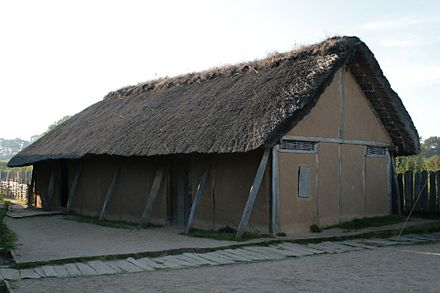
\includegraphics[width=0.33\textwidth]{aussen.jpeg}
  Ein Wikingerhaus von außen.
\end{wrapfigure}

Das Hauptmaterial war Holz, aber es wurde auch Stein, Lehm oder Torf benutzt. Von außen wurden die Wände durch Baumstämme gestützt, zudem dienten Gras- und Steinwälle zur besonderen Stabilisierung. Die Dächer waren abgerundet, flach und hatten nur an einer Stelle ein Loch, das für Licht und frische Luft sorgte, aber auch als Abzug für den Rauch des Feuers, das im Inneren des Hauses entzündet wurde, fungierte, denn in die Häuser waren oft keine Fenster eingebaut.


\begin{wrapfigure}{l}{0.35\textwidth}
  \centering
  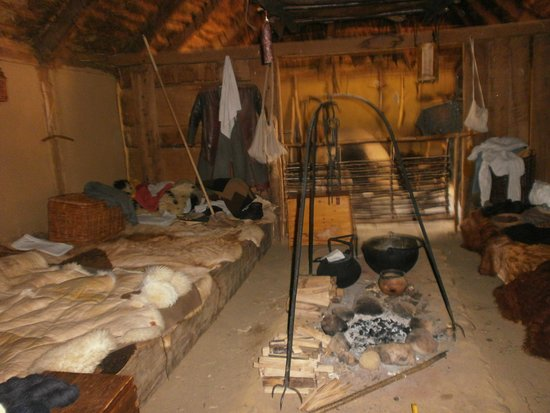
\includegraphics[width=0.33\textwidth]{innen.jpeg}
  Ein Wikingerhaus von innen.
\end{wrapfigure}

Das Innere der Gebäude war meist ein einzelner, großer Raum, in dem sich die Bewohner hauptsächlich aufhielten. Dort wurde gekocht und gegessen, beisammen gesessen, geschlafen und auch gearbeitet. Als Kochstelle diente ein Feuer in der Mitte des Raumes. Außerdem wärmte es die Bewohner des Hauses im Winter. Daneben waren jedoch nicht viele weitere Möbel vorhanden. Es gab Stühle und Bänke, aber manchmal fehlte schon ein richtiger Tisch in manchen Häusern. Als Betten waren Erhebungen oder Nischen bei den Wänden vorgesehen, teilweise gab es aber auch einen kleinen, separaten Raum für die Hausherren zum Schlafen. Geschlafen wurde auf Tierfellen und Stroh. Die Wände waren geschmückt mit Tierfellen, Stoffen, Waffen und Errungenschaften von Seefahrten.

Bei den Wikingern wurde morgens meistens ein nahrhaftes Frühstück gegessen, die nächste Mahlzeit wurde oft erst abends wieder gegessen. Die Nahrung der Wikinger baute auf Nutztieren und Wildtieren auf. Die Tiere waren für die Wikinger die Hauptnahrungsquelle in Bezug auf Fleisch und die Produkte, die die Tiere produzieren, zum Beispiel Milch. Auch erzeugten sie Butter, Käse und Honig. \\
Zum einen diente die Fischerei zur Ernährung der Wikinger. Da die Wikingerdörfer oft an einem Gewässer lagen, war es mit relativ wenig Aufwand verbunden, die gewinnbringenden Fische zu fangen. Zum anderen waren die Nutztiere im Dorf eine Quelle für Nahrung. Fleisch wurde jedoch eher selten konsumiert, da es ein Luxusgut war, dessen Verzehr und Zubereitung mit mehr Aufwand verbunden war. Manchmal gingen die Wikinger auch auf die Jagd, zum Beispiel in Wäldern, und verzehrten die dort erlegten Tiere.
Neben den fleischhaltigen Lebensmitteln ernährten sich die Wikinger auch noch von Getreide und Erzeugnissen daraus. Die Wikinger bauten das Getreide auf ihren eigenen Feldern an und und verarbeiteten es später zu beispielsweise Brot oder Brei. Zudem dienten Obst und Gemüse als Nahrungsmittel. Auch diese wurden im Wikingerdorf in kleinen Beeten oder als Bäume angepflanzt.\\
Getrunken wurde hauptsächlich Alkohol. Zu den bekanntesten Getränken zählt Met, ein Getränk, bestehend aus vergorenem Honig mit Gewürzen, der mit Wasser verdünnt wurde. Dieser wurde häufig und in großen Mengen auf Feiern getrunken. Daneben wurde im Alltag auch Bier konsumiert, das aus Hopfen, Gerste oder Hafer gebraut wurde. Zu den wichtigsten Getränken ohne Alkohol zählten Milch und Wasser.

\subsection{Alltagsablauf}
\flettrine{D}{ie Arbeiten in einem Wikingerdorf} waren vielfältig, wodurch es viele verschiedene Berufe in einem Wikingerdorf gab.
Gearbeitet wurde täglich fast den ganzen Tag lang, wobei sie im Sommer aufgrund der besseren Umstände, zum Beispiel wegen der höheren Temperaturen oder der längeren Tage, länger tätig waren. In der Wikingerfamilie übernahmen schon die Kinder Aufgaben von den Eltern, um ihnen zum einen Arbeit abzunehmen und zum anderen ihre Tätigkeiten besser kennenzulernen, um sie später selbst einmal ausführen zu können.\\
Ein großes Aufgabenfeld war die Tierpflege. Die Nutztiere im Dorf waren für die Wikinger eine Lebensgrundlage, weshalb sich gut um sie gekümmert wurde. Die Tiere wurden jeden Tag gefüttert und deren Ställe gesäubert. Außerdem, auch wenn nicht jeden Tag, wurden zum Beispiel die Kühe oder Ziegen gemolken, die Schafe geschoren und die Daunen der Gänse wurden gerupft.\\
Im Zusammenhang mit den Tieren steht auch die Feldarbeit, die auch zu den täglichen Arbeiten gehörte, denn die Ochsen zogen die Pflüge und unterstützten die Wikinger bei schweren Arbeiten. Die Felder wurden im Frühjahr bepflanzt, im Herbst bis Spätherbst dann geerntet. Die Felder waren auch Lebensgrundlage für ein Wikingerdorf, weshalb die meiste Arbeitszeit in die Instandhaltung dieser investiert wurde. Neben diesen grundlegenden Aufgaben, die meist von allen Bewohnern des Dorfes ausgeführt wurden, gab es auch einige Handwerksberufe.
Zu den Grundlagen der Handwerkskunst der Wikinger gehörte zum Beispiel das Schnitzen,
Weben oder Bauen. So gut wie alle Gegenstände, die im Leben der Wikinger Gebrauch
fanden, von Besteck bis Kleidung, waren selbst gefertigt, weshalb es für die Wikinger sehr
wichtig war, dass die Meisten die Techniken beherrschten. Vor allem die Frauen waren in
der Herstellung von Kleidung und anderen Sachen tätig. Sie übernahmen oft auch die Arbeit der Männer, wenn diese auf der See unterwegs waren.
Zudem gab es einen oder mehrere Schmiede, die für Arbeiten an Tieren nötig waren, zum Beispiel an den Hufen der Tiere, aber auch für Schmiedearbeiten mit Eisen, zum Beispiel bei der Fertigung von Schwertern, die dann später im Kampf genutzt werden konnten. Außerdem gab es ein oder mehrere Schiffsbauer, die für die Konstruktion und Verbesserung der Schiffe zuständig waren.\\
Auch zu erwähnen ist der Bereich des Handels: Die Wikinger waren gute Händler und handelten mit Gütern aus dem Dorf oder welchen die bei Plünderungen geraubt wurden. Gehandelt wurde auf Märkten in der Nähe des Dorfes oder Übersee, so kamen die Wikinger auch in den Besitz von fremdländischen Handelsgut, wie zum Beispiel Stoffe.\\
Nach der Arbeit begann die Freizeit der Wikinger, die sie gerne mit Spielen, Bewegung oder anderen Freizeitbeschäftigungen vertrieben.
Mit spielerischen Zügen wurde das Kämpfen auch in der Freizeit geübt und manchmal auf kleineren Turnieren innerhalb des Dorfes ausgeweitet. Dabei wurde der Umgang mit Schwertern, Pfeil und Bogen oder Speeren geübt, außerdem wurde das Reiten gleichzeitig eingebunden. Eine weitere Beschäftigung waren Spiele, insbesondere Brettspiele oder Ballspiele. Zum Beispiel fanden Archäologen ein Brettspiel, das an unser heutiges Spiel \glqq Mühle\grqq{} erinnert, aber auch ein anderes, welches Schach ähnelt. Das Ballspiel \textit{knattleikr}, ähnlich zum heutigen irischen Schlagballspiel \glqq Hurling\grqq{}, war außerdem weit verbreitet. Die Kinder hatten oft auch Spielzeuge aus Holz, die in der Freizeit gefertigt wurden. Im Winter nutzten sie den Schnee und das Eis, um Schlitten zu fahren und Schlittschuh zu laufen.\\
Die Wikinger waren ein sehr geselliges Volk, weshalb sie meistens ihre Freizeit in Gruppen verbrachten.
Vor allem die Männer saßen abends gerne zusammen an einem Tisch und tranken zusammen Bier, dadurch ehrten sie ihren Gott. Es wurde Musik gespielt und dazu getanzt, außerdem wurde sich viel unterhalten. Die Musik wurde auf Instrumenten wie Trommeln, Flöten und verschiedensten Zupfinstrumenten gespielt.


\aufgaben{
  \item Nutze die Informationen aus dem Text und schildere deinen Tagesablauf in einem Tagebucheintrag.
  \item Vergleiche die Informationen aus den Texten mit deinen Erwartungen und nenne Beispiele, wie sich der Alltag zu heute verändert hat.
}

\fchapter{Wikinger um die Welt}

\section{Geografischer Überblick}
\begin{center}
  \hspace*{-2.35cm}
  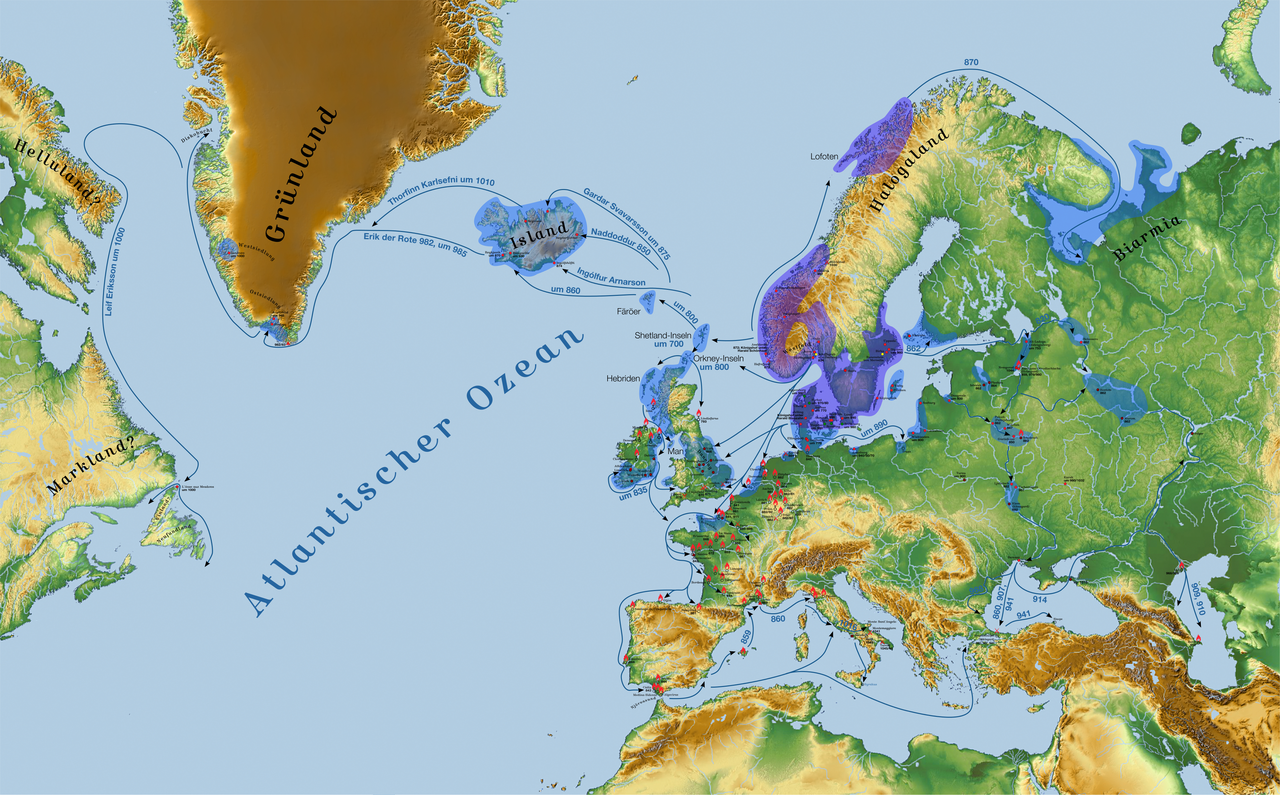
\includegraphics[width=0.9\paperwidth]{siedlungspunkte.png}
\end{center}

\textbf{Normandie}\\
In der Vergangenheit gab es immer wieder Angriffe auf das Frankenreich. Ab dem Jahre 879 n. Chr. brach dann jedoch eine große Flut von Überfällen über die Franken herein. Die Wikinger kamen mit hunderten Drachenbooten, welche mit tausenden Kriegern bemannt waren. Sie plünderten und zerstörten zahllose Dörfer, Städte und Klöster. Einer der bekanntesten Ereignisse dieser Zeit war der Angriff auf Paris (885-886 n. Chr.). Es war eine sehr blutige Schlacht mit vielen Toten auf beiden Seiten.
Am Ende plünderten die Wikinger Paris, zogen jedoch wieder ab.

\textbf{Island}\\
Im Jahre 850 n. Chr. erreichte der Wikinger \textit{Naddoddur} als erster durch Zufall die Insel Island. Eigentlich lag sein Ziel woanders, er kam jedoch vom Kurs ab und landete auf Island. Später entdeckten und besiedelten dann Wikinger wie \textit{Gardar Svarsson} und \textit{Ingólfur Arnason} das Land. Es bildeten sich schnell Siedlungen und viele Wikinger, die in ihrem Land nicht erwünscht waren, sahen in Island eine Lösung für einen Neuanfang. Die erste größere und älteste Siedlung war Reykjavik (870 n. Chr.). 

\textbf{Grönland}\\
Von Island war es nicht weit nach Grönland und schon bald wurden die Segel in diese Richtung gesetzt. \textit{Erik der Rote} hat um das Jahre 882 n. Chr. als erster Wikingerführer Grönland entdeckt. Er musste aus Island fliehen, da er dort wegen Totschlags geächtet wurde. Er überzeugte viele andere, mit ihm zu kommen und gründete mit ihnen einige Siedlungen. Sie lebten von Handel, Viehzucht, Ackerbau und Fischerei. Obwohl es circa 250 Siedlungen gab, waren die Wikinger um 1550 schon wieder aus Grönland verschwunden. Die Gründe dafür sind umstritten, jedoch lag es wahrscheinlich an Krankheiten und den Klimaverschlechterungen seit dem 14. Jahrhundert.

\textbf{Amerika}\\
Als erster Wikinger (und wahrscheinlich auch Europäer) entdeckte \textit{Leif Eriksson}, der Sohn von \textit{Erik dem Roten}, um das Jahr 1000 n. Chr. Amerika. Er landete dort zunächst in Neufundland, damals nannte er es \textit{Vinland}, und versuchte dort eine Siedlung aufzubauen. Nachdem er nach Grönland zurückkehrte, fuhr als nächstes sein Bruder \textit{Thorwald} dorthin. Dieseieser versuchte ebenfalls zu siedeln, hatte aber einige gewaltvolle Auseinandersetzungen mit den Einheimischen, in denen er schließlich getötet wurde. Die Wikinger blieben daraufhin aus Amerika fort.

\textbf{Mittelmeerraum}\\
Unter der Führung von  \textit{Bjǫrn Ragnarsson járnsíða} und \textit{Hástein} um 840 n. Chr. kamen die Wikinger mit einer Flotte über Spanien ins Mittelmeer. Sie plünderten und zerstörten viele Klöster, Städte und Dörfer. Um 860 n. Chr. erreichten sie über die Mittelmeerküste des Frankenreichs Italien. Sie wollten die große Stadt Rom plündern, verwechselten sie jedoch mit einer nördlichen Stadt namens Luna. Danach segelten sie sogar über Konstantinopel bis ins Schwarze Meer, bevor sie sich auf die Heimreise machten. Um 1000 n. Chr. gab es eine neue Angriffswelle der Wikinger in Süditalien. Sie griffen Rom an und raubten zahlreiche Besitztümer aus  süditalienischen Städten und Dörfern.
Danach waren die Wikinger auch dem Mittelmeer ferngeblieben.

%TODO hier noch eine aufgabe?

\section{Die Wikinger in England}
\flettrine{M}{it dem Angriff der Wikinger} 793 n. Chr. auf das Kloster der Insel Lindisfarne brach eine neue Ära der Wikingerzeit an. Sie raubten die Besitztümer des Klosters, töteten die Priester und zerstörten das Kirchengelände. Es folgten weitere Plünderungen im Norden Englands, welche jedoch nicht sehr bedeutend waren. Die Wikinger blieben dann 30 Jahre aus England fern. \\
Im Jahre 835 n. Chr. namen die Angriffe eine neue Dimension an. Ihre Angriffe konzentrierten sich jetzt mehr auf den Süden, waren größer und häuften sich. Außerdem kamen sie nicht mehr nur im Sommer, sondern überwinterten. So mussten die Menschen auch im Winter Angst vor Angriffen haben. \\
Um nicht den stetigen Angriffen der Wikinger ausgesetzt zu sein, fingen Fürsten und Könige an ihnen das sogenannte \textit{danegeld} zu zahlen. Dies waren Zahlungen damit sie verschont blieben.
851 n. Chr. wurden die Wikinger das erste mal von König Ethelwulf in einer größeren Schlacht geschlagen und vertrieben.

\begin{center}
  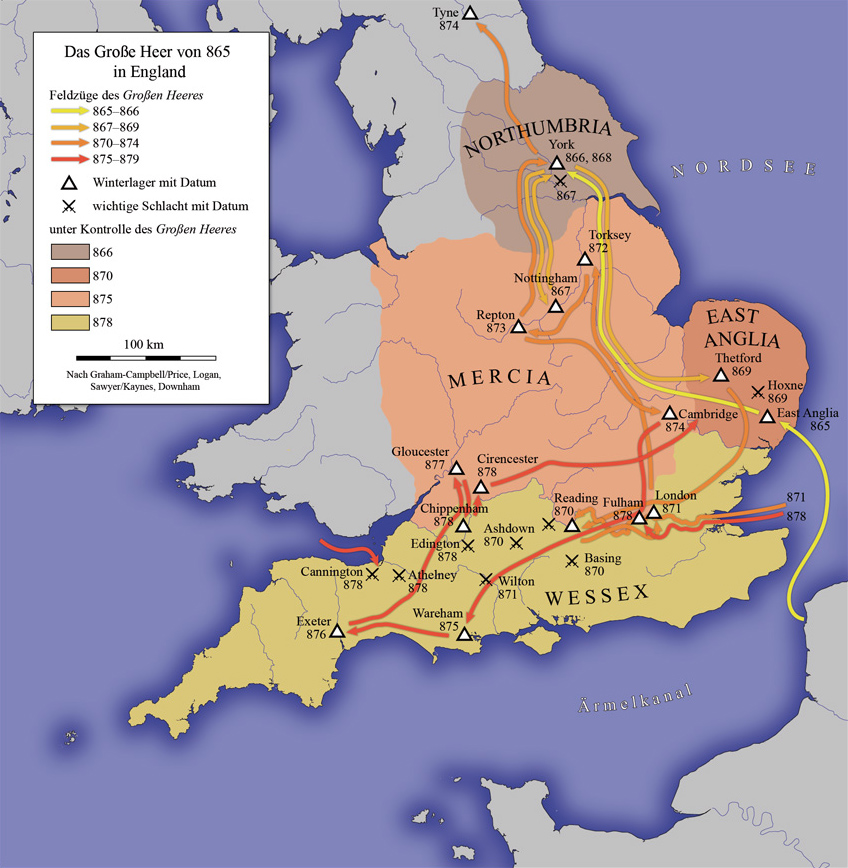
\includegraphics[width=0.9\textwidth]{england865.png}
\end{center}

Einige Jahre später veränderte sich das Geschehen gänzlich. Die Wikinger kamen 865 n. Chr. mit einer riesigen Armee, genannt \glqq Das große Heidenheer\grqq{}, dem fast niemand trotzte. Angeführt von Ivar dem Knochenlosen und seinen Brüdern, eroberten sie 866 n. Chr. die Hauptstadt von Northumbria, York. Dann zogen sie weiter, besiegten 869 n. Chr. Eastanglia und eroberten 874 n. Chr. ein Teil von Mercia. Das Wikingerreich \textit{Danelag} war gegründet. Die Wikinger hatten erstmals nicht nur sporadische Plünderungen gemacht, sondern ein ganzes Gebiet in England erobert. \\
Nun stand ihnen nur noch ein größeres Reich im Wege, um ganz England zu erobern. Das Königreich Wessex im Süden, unter der Führung von König Alfred. Den Wikingern kam \glqq das große Sommerheer\grqq{} unter der Führung von König Guthorm zur Unterstützung. Die Heere verbündeten sich und lieferten sich einige Schlachten mit dem Heer von Wessex. \\
878 n. Chr versammelte König Alfred ein noch größeres Heer und schlug das große Wikingerheer endgültig in die Flucht.
Bis 899 n. Chr. gab es weitere Versuche von großen Heeren, Wessex zu besiegen. König Alfred schaffte es jedoch, bis zu seinem Tod die Wikinger immer wieder zu vertreiben.\\\\
Bis 954 n. Chr. schaffte es Wessex das Danelag einzunehmen und die Wikingerführer aus England zu vertreiben. Die Wikinger wurden zwar vertrieben, kamen jedoch 30 Jahre später erneut mit Armeen unter der Führung von Sven Gabelbart, um zu plündern und zu rauben. Wieder gab es viele Jahre des Krieges. Sie schafften es, viele Teile von Wessex, Mercia, etc. einzunehmen und den damaligen König Ethelred zu besiegen. Es folgten Jahrzehnte des Krieges, der Intrigen und der Korruption. Nachdem der Wikingerführer Harold Godwinson Anspruch auf den Thron erhob, kam es am 25. September 1066 zur Schlacht von Stamford Bridge. Dort wurden die Wikinger vernichtend geschlagen und blieben England fortan fern.

\aufgaben{
  \item Lies den Text und erstelle eine Chronologie der Ereignisse.
  \item Begründe, warum England für die Wikinger als Angriffsziel so attraktiv war.
}

\fchapter{Die Wikingergesellschaft}

\section{Ständeordnung}
\flettrine{B}{ei den Wikingern} gab es einen starken Bezug zur Götterwelt, im Glauben und auch im Alltag.
Laut den Sagen gab es drei Stände: Die Sklaven, die Freien und die Jarls.
Diese drei Gesellschaftsklassen sind unter anderem durch das sogenannte Lied oder Gedicht von \erklaer{\textit{Ríg}}{Auch Heimdall genannt. Schutzgott und Gott des Morgenlichtes.} (auch genannt \textit{Rígsþula}) begründet. Darin wird beschrieben, welche Tätigkeiten die jeweiligen Standesmitglieder ausüben und wie diese aussehen.
Die Sklaven haben beispielsweise einen krummen Rücken und ein schreckliches Aussehen, wohingegen die Bauern rote Haare haben und mit Tieren arbeiten. Die Jarls, beziehungsweise der Adel, haben helles Haar, leuchtende Wangen und herrschen über ihr Gebiet.
Da die oben genannten Vorstellungen einer mytischen Götterwelt entstammen, gab es in der Realität einige Unterschiede.
Zuerst muss man sagen, dass der Begriff \glqq Sklave\grqq{} bei den Wikingern leicht anders ist als unsere typische Vorstellung eines Sklaven. Sie wurden zwar auch gehandelt (zum Beispiel in Haithabu), jedoch konnten sie sich mit Arbeit auf einem Wikingerhof freiarbeiten oder freikaufen, wenn man das Geld hatte, sodass die Sklaven bei den Wikingern sozusagen wieder frei werden konnten.\\\\
Die größte und breiteste Schicht waren die Freien, sie waren die normalen Wikinger, oft auch \textit{bóndi} genannt. Zu ihnen zählten Bauern, Fischer, Handwerker, Kaufmänner und auch Seenavigatoren, somit übten sie ein vielfältiges Betätigungsfeld aus.
Es gab jedoch auch Berufe, welche eine gewisse Spezialisierung brauchten. Dazu zählte zum Beispiel der Arzt, welcher ein Wissen über (natürliche) Heilkunde besaß, diese Tätigkeit wurde übrigens meist von Frauen ausgeführt. Auch gab es den \glqq Schmied\grqq{} beziehungsweise eher den besonders talentierten Handwerker, welcher oft bewundert wurde, denn er konnte - wie die Götter - etwas erschaffen, obwohl die Maßstäbe verschiedene waren.
Außerdem gab es noch eine Art \glqq Priester\grqq{} oder Geistlichen, welcher zum Beispiel Zeremonien und bestimmte Feste leitete. Jedoch konnte diese Tätigkeit auch von Personen ausgeübt werden, die einen guten Ruf besaßen.
Allgemein war es aber untypisch sich auf einen Beruf zu spezialisieren, der Wikinger war ein eher vielfältiges Multitalent.
Besonders war auch, dass die Wikinger schon ein starkes Bewusstsein für Gerechtigkeit hatten und es so auch \textit{bóndi} gab, welche gewissermaßen als Anwälte andere beraten haben. Wenn jemand durch einen anderen benachteiligt wurde, klagte dieser sein Recht ein und er wurde gegebenenfalls entschädigt oder der Schuldige bestraft. Weiterführend gab es auch die bereits erwähnte öffentlichen Versammlung \glqq Thing\grqq{}. Hier war es dem \textit{bóndi} möglich, frei seine Meinung zu sagen. Durch dieses Recht durfte er sogar selbst dem König gewissermaßen (eingeschränkt) widersprechen. Das Forum bot zudem auch eine Diskussion über allgemeine und öffentliche Angelegenheiten bezüglich der Gesetze, der Rechtsprechung und des Handels.
Obwohl die Freien sehr breit definiert waren, gab es noch eine Unterscheidung nach Wohlstand und Ansehen in der Gesellschaft. Demnach gab es die sogenannten großen (\textit{stórbœndr}) und kleinen (\textit{smábœndr}) bóndi. 
Der große \textit{bóndi} zeichnet sich somit zum Beispiel durch seine Familie, welche sehr alt und respektiert war, aus. Zudem war er eher wohlhabend und genoss wahrscheinlich bestimmte Privilegien, da seine Familie in der Gesellschaft besonders respektiert wurde.\\\\
Die Könige, welche meist auf einer sehr lokalen Ebene geherrscht haben und deswegen nicht mit den mittelalterlichen Königen vergleichbar sind, wurden aus den Reihen der \textit{stórbœndr} von den anderen \glqq großen\grqq{} \erklaer{\textit{bœndr}}{Plural von \textit{bóndi}.} gewählt. Bei dieser Zeremonie stieg der Gewählte auf einen heiligen Stein und absolvierte einen königlichen Lauf. Wenn dieser nicht den Erwartungen entsprach, wurde der Kandidat vom Stein gestürzt. Doch wenn er bestand, wurde er König über eine Region, die meist ungefähr einen Fjord oder Gebirgszug umfasste.
Über die Jarls hingegen ist weniger bekannt, so ist beispielsweise das Verhältnis zwischen Jarl und König nicht genau geklärt, jedoch hatte er einen geringen Rang als der König. Der König ernannte eine Person zum Jarl, wenn diese ihm besondere Dienste geleistet oder anderweitig seinen Respekt erlangt hatte.

\aufgaben{
  \item Beschreibe das Gesellschaftsleben der \textit{bóndi} in einem Text.
  \item Begründe, ob du dich in der Wikingergesellschaft wohlfühlen würdest und beziehe Sichtweisen aus den verschiedenen Ständen ein.
  \item Bewerte die Fairness und soziale Mobilität (Beweglichkeit in Bezug auf die soziale Stellung) in der Gesellschaft.
}

\section{Gemeinschaft und Gesellschaftsbild}
\flettrine{D}{er Wikinger} hat selbst sich nicht als Individuum, sondern als Teil einer Gemeinschaft definiert. Beispielsweise über seine Familie, Verwandte und Ahnen. Diese Zugehörigkeit zu einer Sippe war enorm wichtig für die Wikinger und musste nicht nur im Familienkreis bestehen, im Gegenteil, ein Zusammenschluss war in vielen Beziehungen angestrebt. Der Gemeinschaftsgeist war so stark ausgeprägt, dass unter anderem das Vermögen oder die Ressourcen des Einzelnen auch oft - zum Wohl der Gemeinschaft - dieser zugewendet wurden. Als Anekdote kann man hier anführen, dass dies teilweise auch an den altnordischen Wörtern für legen (in bestimmt konjugierter Form \textit{lag}), Vermögen (\textit{fé}) und Gemeinschaft (\textit{félag}) deutlich wird. Diese Gemeinschaften bilden dann auf einem räumlich begrenzten Raum ein \textit{land}.

Die Familie umfasste bei den Wikingern neben Verwandten auch enge Freunde,
Schwurbrüder und Hausangestellte. Diese Großfamiliengemeinschaft enthielt meist circa 50 Personen, die somit ein Verhältnis zu dem Familienoberhaupt (\textit{húsbóndi}) und seiner Frau, der \textit{húsfreyja}, hatten.\\
Wenn man blutsverwandt war, definierte man sich auch nicht über einen Familiennamen, sondern darüber, dass man Sohn oder Tochter des Vaters war. Dies wurde durch den Anhang -son (Sohn von) und -dóttir (Tochter von) hinter dem Vornamen angemerkt.
Wodurch wieder betont wird, wie wichtig eine gewisse \glqq Zugehörigkeit\grqq{} ist. Weiterführend galt unter den \textit{bóndi} das auswendige Aufzählen der Ahnenreihe als Tugend und war oft sogar eine gesetzliche Pflicht.

\textbf{Familienleben}\\
In der Wikingergesellschaft war der engere Familienkreis mit meist fünf bis sechs Mitgliedern das am häufigsten auftretende Gefüge. Diese, aber auch mehrere einzeln zusammenlebende Personen, bildeten einen Haushalt. Größere Familien gab es oft auch nur als Zusammenschluss von zwei Familien oder in Gebieten oder Professionen, die eine Vereinigung begünstigten (wie zum Beispiel die Tierhaltung). Zudem wohnten die Verwandten und Hausangestellten auch oft mit der Kernfamilie in einem Haus, sodass dieser Haushaltsverbund häufig 10 bis 13 Personen umfasste. Jedoch war vor allem bei ärmeren Bauernfamilien die Familie eher klein.

\textbf{Heirat}\\
Vor der \erklaer{\textit{Christianisierung}}{EEE} Skandinaviens war die Heirat zwischen Mann und Frau eine Vereinbarung zwischen zwei Familien, das heißt, dass kaum aus Liebe geheiratet wurde. Eine Heirat diente somit dem Zweck, die Stellung der eigenen
Familie zu bessern, sodass das Verheiraten zweier Personen eine strategische Angelegenheit war. Zudem waren die beiden Ehepartner fast ausschließlich vom
selben Stand und Wohlstand. Wenn es einen Unterschied gab, hielt die Frau meist den höheren Stand inne. Für einen männlichen Wikinger wäre die Heirat zu einer Frau eines niedrigeren Standes absurd, denn das wäre ein mannamunr (ein \glqq Unterschied zwischen den Leuten\grqq{}).\\
Der Heiratsvorschlag konnte immer nur von der Familie des Mannes kommen, genauer vom Mann selbst oder seinem Vater. Wenn der Vorschlag akzeptiert wurde, starteten die Verhandlungen über den Betrag, den die Familie des Mannes zahlen musste und die Mitgift,
die von der anderen Familie gezahlt wurde. Wegen dieser \erklaer{Mitgift}{Gegenstände oder Geld, das einer Frau bei der Heirat von den Eltern mitgegeben wird.} waren Mädchen unter
anderem auch unbeliebter als Jungen.
Bei solchen Verhandlungen hatte die zukünftige Braut, welche oft noch jugendlich war, kein Zutrittsrecht, geschweige denn Mitspracherecht, dies hatten sie erst nach der Christianisierung.
Häufig kam es auch zu Scheidungen, welche von Mann oder Frau vor Zeugen eingeleitet werden konnten. Nach der Christianisierung konnten diese nur noch von Bischöfen genehmigt werden.
Generell durfte die Braut dann aber zum Elternhaus zurückkehren, ebenso wie die Mitgift,
ihr Eigentum und - wenn der Ehemann der Grund für die Scheidung war - der Betrag, den seine Familie als \glqq Brautpreis\grqq{} gezahlt hatte.

\textbf{Kinder}\\
Ein Kind war man in der Wikingergesellschaft nur bis zum 12. Lebensjahr, danach wurde
man von der Gesellschaft als Erwachsener beziehungsweise Erwachsene anerkannt. Somit
mussten die Jugendlichen ab diesem Zeitpunkt die Pflichten eines Erwachsenen tragen. In der Kindheit wurde unter anderem mit Spielzeugen wie zum Beispiel modellierten Waffen oder Tieren gespielt, welche den späteren Alltag als Erwachsener gewissermaßen reflektierten.\\
Die (späteren) Pflichten unterschieden sich je nach Stand, so waren diese für Mädchen aus wohlhabenderen Familien beispielsweise Management- oder Verwaltungstätigkeiten, während Mädchen eines niedrigeren Standes Haushaltsaufgaben wie Kochen oder Waschen erlernten. Bei Jungen waren die Aufgaben zum Beispiel auf Tierherden aufpassen oder, für den Nachwuchs aus reicheren Familien, die Jagdkunde zu erlernen. Gelernt haben sie wahrscheinlich bei den Eltern.

\textbf{Ältere}\\
Senioren gab es unter den Wikingern nicht wirklich, nicht zuletzt aufgrund eines
fehlenden Medizinwesens, mangelnder Hygiene, etc. Durchschnittlich starben die Wikinger
den natürlichen Tod mit 40, nur sehr vereinzelt gab es Personen, die sehr alt wurden, welche aber wahrscheinlich wohlhabend waren. Allgemein war der natürliche Tod durch Altersschwäche oder Krankheit keine beliebte Art zu sterben; man wollte im Gefecht, auf dem Schlachtfeld sein Leben lassen, gewissermaßen \glqq in Ehre\grqq{} sterben. Diese Ansichten entsprangen wahrscheinlich dem Heldenkult der Wikinger, denn ein Held stirbt meist nie durch Altersschwäche. Außerdem gibt es Berichte aus Schweden, in denen die Alten der Familie in Zeiten von Hungersnöten von der Klippe gestoßen wurden oder ihnen mit einem Knüppel auf den Kopf gehauen wurde. Daraus kann man schließen, dass das \glqq Altsein\grqq{} in der Wikingergesellschaft unbeliebt war, auch da man nicht mehr so viel Arbeit verrichten konnte.

\textbf{Brüderschaften}\\
Neben der Familie hatten auch Bluts- und Schwurbrüder eine besondere Stellung, denn
durch das Vermischen des Bluts wurde ein künstliches Verwandtschaftsverhältnis aufgebaut,
wodurch man sozial abgesicherter war. Das genaue Ritual ist dabei nicht bekannt, es sind mehrere überliefert, jedoch wird immer ein Kontakt zwischen dem Blut hergestellt. Dieser Kontakt konnte direkt, indirekt (beispielsweise mit Erde vermischt) oder spirituell (in Fußspuren träufeln) passieren. Blutsbrüderschaften konnten auch mehrere Personen umfassen, sodass sich sozusagen ein Verbund bildete.
Dabei bestand immer eine Rachepflicht, das heißt, dass man den Blutsbruder rächen musste. Mit der Christianisierung wurde die Blutsbrüderschaft weniger brutal und wandelte sich eher zu einer Schwurbrüderschaft. Bei dieser wurde die Rachepflicht zum Beispiel durch Forderungen nach Entschädigungszahlungen abgelöst.

\aufgaben{
  \item Vergleiche die in dem Text beschriebenen Aspekte mit deinem heutigen Sozial- und Gemeinschaftsleben.
  \item Beurteile ob \glqq Gemeinschaft\grqq{} heute noch so einen hohen Stellenwert wie bei den Wikingern hat und inwiefern sich der Begriff gewandelt hat (z.B. durch Social Media).
}

\section{Die Rolle der Frau}
\flettrine{N}{atürlich} machten nicht nur die Männer die Zivilisation der Wikinger aus, sondern auch die Frauen waren ein Teil dessen, und zwar gewiss kein unwichtiger. Sie wurden \textit{húsfreyja} genannt. Während die Männer teilweise mit den Söhnen auf Raubzug waren, blieben die Frauen und Mädchen in der Sippe zurück. Und daheim fielen auch so einige Aufgaben an, die bewältigt werden mussten.\\
Die Frauen waren während der Absenz der Männer die Leitung der Sippe und ein Symbol für ihre Autorität waren die Schlüssel, die an ihren Gürteln befestigt waren. Sie waren die Herrin des Hauses. Dafür gab es auch Bezeichnungen wie \textit{innan húss} (im Haus) oder \textit{innan stokks} (innerhalb der Türschwelle).\\
Mit dieser Befehlsgewalt war es beispielsweise eine ihrer Aufgaben, die Sklaven zu befehligen. Für diese Sklaven hatte man auch einen Namen, und zwar \textit{Thrall}, was soviel wie \glqq unreifer Knecht\grqq{} bedeutet. Diese \textit{Thralls} übernahmen die niederen Aufgaben, für dessen Bewältigung es keine besondere Fertig- und Fähigkeit bedurfte. 
Genauso waren die Frauen dafür verantwortlich, die Behausung sauber und ordentlich zu halten. Auch wenn die Häuser, in denen die Wikinger lebten, nicht wirklich groß waren,
befand sich dort vieles, das zu putzen war.\\
Auch befand sich dort eine Feuerstelle, an der die Frauen auch das Kochen für die Familie übernahmen. Außerdem stand in dem Raum auch oftmals noch ein Webstuhl, an dem die Frauen Kleider und Gewänder anfertigten. Aus der gesponnenen Wolle webten sie Tücher, die sie unter anderem auch zu Wandbehängen oder Bezügen für Wandbänke nähten. Auch aber stellten sie die riesigen Segel für die Schiffe der Männer her.
Ebenso war es die Aufgabe der Frau, die Kinder zu erziehen und zu beschäftigen, auch wenn die Erziehung je nach Geschlecht von den jeweiligen Elternteilen übernommen wurde.
Schließlich musste die Frau ebenfalls das Vieh füttern, pflegen und auch beherbergen, was auch von besonderer Wichtigkeit war, gerade weil damit beispielsweise Handel betrieben wurde.\\\\
Aber nicht nur die Aufgaben und Pflichten fielen für die Frauen an, sondern sie hatten auch viele Rechte. Zum Beispiel hatten sie die Möglichkeit, sich von ihrem Ehemann scheiden zu lassen, wenn es ihr Wille war. Durch eine starke Nachbarschaftsgemeinschaft war die Frau stets unterstützt. Dies spricht für die Unabhängigkeit der Frau und für ihren gleichwertigen Stand gegenüber dem Mann. Dennoch durfte sie sich vor dem Recht nicht selbst vertreten und sie hatte kein wirkliches Mitspracherecht in der Politik. Aber das soll nicht den Eindruck erwecken, dass die Wikingerfrau sich nicht anderweitig zu behaupten wusste.\\
Sie war sogar sehr wohl ein bedeutender Teil der Handelsgesellschaft. Sie übernahm nämlich das Wiegen und Gewichten der Waren. 
Auch waren Frauen in der Wikingerzeit in der Lage, einen Hof zu besitzen. Dies war jedoch vom jeweiligen Fall abhängig. War eine Frau verwitwet, also ihr Mann war vermutlich auf einem seiner Raubzüge gestorben, so konnte sie durchaus den gemeinsamen Hof erben und der wurde dann nach ihr benannt. Das Recht zu erben war also aus heutiger Sicht eines, das für eine große Unabhängigkeit spricht.\\\\
Alles in allem kann man also sagen, dass die Wikingerfrauen in Hinsicht auf ihre Rechte und ihr Ansehen gesellschaftlich gut gestellt waren, jedoch in der Politik noch immer nicht viel zu sagen hatten. Im Vergleich aber auch zu anderen Kulturen (gegebenenfalls zur selben Zeit) waren jene noch lange nicht so entwickelt und modern engagiert, wie es die Kultur der Wikinger zu damaliger Zeit war:
Die Frau wurde als vollwertiger und etablierter Teil der Gesellschaft angesehen.

\aufgaben{
  \item Fasse die Aufgaben der Frau zusammen.
  \item Bewerte mithilfe deiner Notizen zu voriger Aufgabe die Rolle der Frau (z.B. in Bezug auf Gleichberechtigung).
  \item Arbeite Gemeinsamkeiten und Unterschiede in Gegenüberstellung zu der Frau heute heraus.
}

\fchapter{Schluss}

\section{Zusammenfassung}

\setstretch{1.3} % 1.3x line spacing zum ausfüllen

\flettrine{D}{Das Wikingerzeitalter} erstreckte sich über die Jahre zwischen \luecke{7.} und \luecke{10.}. Es fanden sich Männer aus dem \luecke{skandinav} zusammen, also Dänemark, Norwegen und Schweden und gemeinsam ergaben sie ein buntes Gemisch aus verschiedensten Individuen. Darunter waren nicht nur Kämpfer, sondern auch \luecke{Händl}, \luecke{Baue}, \luecke{Seemänn} und \luecke{Siedle}. Einer der heutzutage bekanntesten Orte, den die Wikinger besiedelt hatten, ist die ehemalige Handelsstadt \luecke{Haithabu}. Sie diente durch ihre günstige Lage zwischen Nord- und Ostsee als Hauptumschlagplatz für verschiedenste Waren.
Bevor sich die Wikinger zwischen 900 und 980 in Skandinavien niederließen, ereigneten sich jedoch noch einige historisch festgehaltene Ereignisse. Die Wikinger waren bekannt für ihre \luecke{Raubzüge} und sie bereisten mit ihren Schiffen so einiges Gewässer. Ein Meilenstein in der Geschichte der Wikinger sind die Plünderungen in \luecke{England} gewesen. Die Ära der Schlacht um England begann 793 n. Chr. mit einem Angriff der Wikinger auf \luecke{das Kloster.}, gefolgt von weiteren Angriffen seitens der Wikinger auf England, woraufhin die Fürsten und Könige begannen, den Wikingern zur Besänftigung sogenanntes \luecke{Danegeld} zu zahlen. Noch einige weitere Jahrzehnte führten die Engländer Krieg mit den Wikingern, welche sie zumeist mit Mühe und Not vertrieben, bis die Wikinger schließlich wieder zurückkamen und der Krieg weiter andauerte. Im September 1066 kam es dann jedoch zu der endgültigen und wohl alles entscheidenden \luecke{Schlacht von.}, in der die Wikinger geschlagen und weitestgehend  zurückgetrieben wurden.
Die Gesellschaftsordnung der Wikinger stützte sich auf den starken Glauben an die Götter; somit gab es laut einer Sage genau drei Stände. Die \luecke{Sklaven}, die \luecke{Freien} und die \luecke{Jarls}.
Zudem wurden die \luecke{Sklaven} zwar gehandelt und mussten auf dem Wikingerhof arbeiten, aber sie konnten auch durch \luecke{harte Arbe.} ihre Freiheit zurückerlangen.
Die breiteste Bevölkerungsschicht waren die \luecke{.....}\\
\luecke{bón}. Sie waren vielseitig talentiert und hatten einen besonderen Hang zur Rechtskunde. Andere spezialisierte Tätigkeiten, die auch besonderes Wissen erforderten, waren zum Beispiel \luecke{SchmiedArzt}. Die bœndr wurden unterteilt in \luecke{stórbœn} und die \luecke{smábœn}, ersterer zeichnete sich durch \luecke{hohes Familienansehe.}\\
\luecke{Wohlstand...} aus. Die \luecke{Könige} haben meist über \luecke{eine kleine region} geherrscht und wurden von den \luecke{stórbœndr} gewählt, nachdem der Kandidat \luecke{einen...}\\
\luecke{lauf..}. Wenn jemand dem König besondere Dienste geleistet hatte, ernannte er ihn zum \luecke{Jarl}.
Die Wikingergesellschaft war sehr auf Gemeinschaft fokussiert. Die Zugehörigkeit zu \luecke{einer Sippe} war sehr wichtig für das Individuum. Zugehörig zu etwas konnte man zum Beispiel im Sinne einer Familie oder \luecke{einer Blutsbrüderschaft} sein.
In einer großen Familiengemeinschaft waren so meist ungefähr \luecke{50} Individuen vertreten, es lebten aber meist nur \luecke{10 bis 13} Personen in einem Haushalt.
Die Heirat war damals ausschließlich \luecke{strategisch} motiviert, es gab eigentlich keine Liebesheirat. Die Frau hatte vor der \luecke{Chris.}\\
\luecke{tian.} bei der Heirat kein \luecke{Mitspra.}, konnte sich aber von ihrem Mann scheiden lassen, was in anderen zeitgenössischen Gesellschaften \luecke{ni.}\\
\luecke{ht mögli}.
Nach der Christianisierung hat sich auch der Brauch der Blutsbrüderschaft gewandelt, sie wurde weniger brutal und anstatt den Schuldigen \luecke{umzubringen}, wurde nun zum Beispiel \luecke{Geld} als Entschädigung gefordert.
In den Dörfern der Wikinger standen viele Häuser, die \luecke{Langhäuser} genannt wurden. Diese bestanden zum Hauptteil aus \luecke{Holz}. Ihre Konstruktion war perfekt an die Umweltbedingungen angepasst. Im Inneren war meist nur ein großer \luecke{Hauptr.}. Dort fanden die Hauptaktivitäten gemeinsam statt. Vor allem das Essen, das zum Großteil aus \luecke{fleischhaltigen Lebens..} und \luecke{Getreide} bestand, wurde dort meist zusammen verbracht. Dieses Essen wurde durch Arbeit, bei der \luecke{jeder} mithalf, auf den Feldern oder mit den Tieren erwirtschaftet. Neben der Arbeit wurde die Freizeit zum Beispiel mit Ballspielen wie \luecke{knattl.}, Musik, Brettspielen wie \luecke{Müh.} oder \luecke{Schac.} oder mit spielerischen \luecke{Kämpfen} verbracht. 
Die männlichen Wikinger trugen im Alltag als Kleidung hauptsächlich eine \luecke{Tu..} und eine \luecke{Hose}. Die Frauen trugen ein Gewand, das einem \luecke{Kleid} ähnelte. Als Accessoires dienten Schmuckstücke wie zum Beispiel \luecke{Bro.}\\
\luecke{sch}. Gefertigt wurde die Kleidung von den \luecke{Fraue.........} durch \luecke{Spinnen} und \luecke{Weben}. Als Stoff wurde zum Beispiel \luecke{Wolle} von den Tieren aus ihrem Dorf genutzt.
\\
Alles in allem ist also zu sagen, dass die Wikingergesellschaft eine sehr weit entwickelte und eine ihrer Zeit durchaus voraus gewesene war gerade in Bezug auf parallel existierende Gesellschaften. 

\aufgaben{
  \item Fülle den Lücketext aus und beweise dein Wissen!
}

\afterpage{\blankpage}

\newgeometry{ % better for listing references
margin=2cm,bottom=2.5cm}
\newpage % für quellen
\section{Quellenangaben}
\urlstyle{same}
\textbf{Cover und Umschlag}\\
- \url{https://www.tvollmer.de/picture.php/9__Wikinger_und_Mittelalterspektakel_20150418-172343_9745}, Creative Commons.\\
- \url{https://commons.wikimedia.org/wiki/File:02015_Wikinger_Reenactment-Gruppen_des_10.Jahrhunderts_-Trzcinica_011.jpg}, Creative Commons.\\
- \url{https://haithabu.de/upload/img/haithabu.jpg}.\\
- \url{https://commons.wikimedia.org/wiki/File:Das_Wikingerdorf_am_Walchensee_(3948148934).jpg}.\\
- \url{https://commons.wikimedia.org/wiki/File:Vinland_Map_HiRes.jpg}.\\

\textbf{Kapitel 1}\\
- \url{https://de.wikipedia.org/wiki/Haithabu}.\\
- \url{https://www.planet-wissen.de/kultur/voelker/wikinger/pwiediegesellschaftderwikinger100.html}.\\
- \url{https://wikinger-online.de/haithabu/}.\\
- \url{https://www.dw.com/de/wikinger-wie-waren-sie-wirklich/a-19106472}.\\
- \url{https://plarium.com/de/blog/wikingergeschichte/}.\\
- \url{https://www.norwik.de/kindererziehung-bei-den-wikinger/}.\\
- \url{https://www.deutschlandfunkkultur.de/welterbe-museum-bei-schleswig-die-welt-der-wikinger-in.1001.de.html?dram:article_id=459012}.\\
- Régis Boyer. Die Piraten des Nordens. Leben und Sterben als Wikinger. Klett-Cotta, 1997, S. 19 - 28.\\

\textbf{Kapitel 2}\\
- Bilder von Klamotten und Waffen sind selbst gemalt.\\
- Boyer, Régis - Die Piraten des Nordens, Paris, 1992.\\
- \url{https://de.wikipedia.org/wiki/Langhaus_(Wohngebäude)#Nordisches_Langhaus} (15.05.2020).\\
- \url{https://klimagerechtesbauen.blogspot.com/2013/09/kaltes-klima-die-hauser-der-wikinger_17.html} (letzter Aufruf: 15.05.2020).\\
- \url{https://www.norwik.de/die-haeuser-oder-haus-der-wikinger/} (letzter Aufruf: 15.05.2020).\\
- \url{http://members.tripod.com/norwegen_online/Hauptframe/Wikingerleben.htm} (letzter Aufruf: 19.05.2020).\\
- \url{https://www.wikiwand.com/de/Wikingerhaus_von_Haithabu}.\\
- \url{https://www.tripadvisor.com/LocationPhotoDirectLink-g11816996-d243443-i336392790-Viking_Museum_Haithabu-Busdorf_Schleswig_Holstein.html}.\\
- \url{https://wikinger-online.de/essen-und-trinken/} (letzter Aufruf: 15.05.2020).\\
- \url{https://www.peraperis.com/blog/bekleidung/die-mode-der-wikinger.html} (letzter Aufruf: 18.05.2020).\\
- \url{http://members.tripod.com/norwegen_online/Hauptframe/Wikingerleben.htm} (letzter Aufruf: 19.05.2020).\\
- \url{https://i.pinimg.com/originals/f3/dc/76/f3dc76541c0ba16b6f89ba64d06afa23.jpg}.\\
- \url{https://www.ribevikingecenter.dk/de/erlebnisse/der-gutshof,-anno-980.aspx}  (letzter Aufruf: 27.11.2020).\\
- \url{https://en.wikipedia.org/wiki/Knattleikr} (letzter Aufruf: 26.11.2020).\\
- \url{http://skagen-larp.de/Foren/Thema/wikinger-berufe/} (letzter Aufruf: 19.05.2020).\\
- \url{https://www.kinderzeitmaschine.de/mittelalter/fruehmittelalter/lucys-wissensbox/wikinger-der-norden/alltag-der-wikinger/} (letzter Aufruf:19.05.2020).\\
- \url{https://www.norwik.de/wikingerzeitliche-spiele/} (letzter Aufruf: 19.05.2020).\\

\textbf{Kapitel 3}\\
- \url{https://commons.wikimedia.org/wiki/File:Z\%C3\%BCge,_Landnahmen_und_Siedlungsgebiete_der_Nordm\%C3\%A4nner_-_800-1050.png}.\\
- \url{https://de.m.wikipedia.org/wiki/Datei:England_Grosses_Heer_865.png}.\\

\textbf{Kapitel 4}\\
- Régis Boyer. Die Piraten des Nordens. Leben und Sterben als Wikinger. Klett-Cotta, 1997, Kapitel 1 und 3.\\
- Kirsten Wolf. Daily Life of the Vikings. Greenwood Press, 2004, S. 7-17.\\

\textbf{Kapitel 5}\\
- \url{https://de.wikipedia.org/wiki/Thrall}.\\
- \url{https://www.norwik.de/kindererziehung-bei-den-wikinger/}.\\
- \url{https://www.miss-jones.de/2019/11/06/die-gleichberechtigung-von-wikinger-und-wikingerin/}.\\
- \url{https://de.wikipedia.org/wiki/Wikingerzeit#Frauen}.\\
- \url{https://www.norwik.de/familienleben-der-wikinger/}.\\
- Boyer, Régis – Die Piraten des Nordens, Paris, 1992.\\

\afterpage{\blankpage}
\newpage
\afterpage{\blankpage}

\thispagestyle{empty}
\setlength{\fboxrule}{1pt} % border for cutting out the images
\setlength{\fboxsep}{5pt} % makes cutting easier

\section{Anhang}

\textbf{Kriegerkleidung}\\\\
\timage{schild.jpeg} \vspace{0.5cm} \timage{tunika.jpeg} \vspace{0.5cm} \timage{hemd.jpeg}\\\\
\timage{speer.jpeg} \vspace{0.5cm} \timage{helm.jpeg}

\pagebreak

\textbf{Waffen}\\\\
\timage{bogen.jpeg} \vspace{0.5cm} \timage{breitaxt.jpeg} \vspace{0.5cm} \timage{handaxt.jpeg}\\\\
\timage{langsax.jpeg} \vspace{0.5cm} \timage{speer2.jpeg} \vspace{0.5cm} \timage{streitaxt.jpeg}\\\\
\timage{wurfaxt.jpeg} \vspace{0.5cm} \timage{suontaka.jpeg}

%\afterpage{\blankpage}
\newpage
\vspace*{24cm} Erstellt von Alexa, Mareike, Nils und William // Projektkurs Wikinger 2020
\thispagestyle{empty}
\newpage
\includepdf[pages=-]{wikinger-workbook-back.pdf}
\thispagestyle{empty}

\end{document}
